\documentclass[11pt,titlepage]{article}
\usepackage{fullpage}
\usepackage{amsmath}
\usepackage{amssymb}
\usepackage{color}
\usepackage{graphicx}
\graphicspath{ {images/} }
\usepackage{tikz}
\usetikzlibrary{shapes,arrows,positioning,calc}
\usepackage{float}
\restylefloat{table}
\usepackage{array}
\tikzset{
	block/.style = {draw, fill=white, rectangle, minimum height=3em, minimum width=3em},
	sum/.style = {draw, fill=white, circle, node distance=1cm},
	input/.style = {draw=none},
	output/.style = {draw=none},
	coord/.style = {coordinate}
}

\author{Rane Brown \\ Kate Schneider}
\title{ECEN 4638: Lab X.1P}
\date{\today}

\begin{document}
\maketitle

\section{Description}
	The purpose of this lab is to explore the torsion disc system and experimentally collect data that will help in the design of a proportional controller. The torsion disc system consists of a platform with three discs aligned above a driving motor. There are various configurations for the torsion disc system and this lab will use a basic setup described below. 
	\begin{figure}[H]
			\centering
			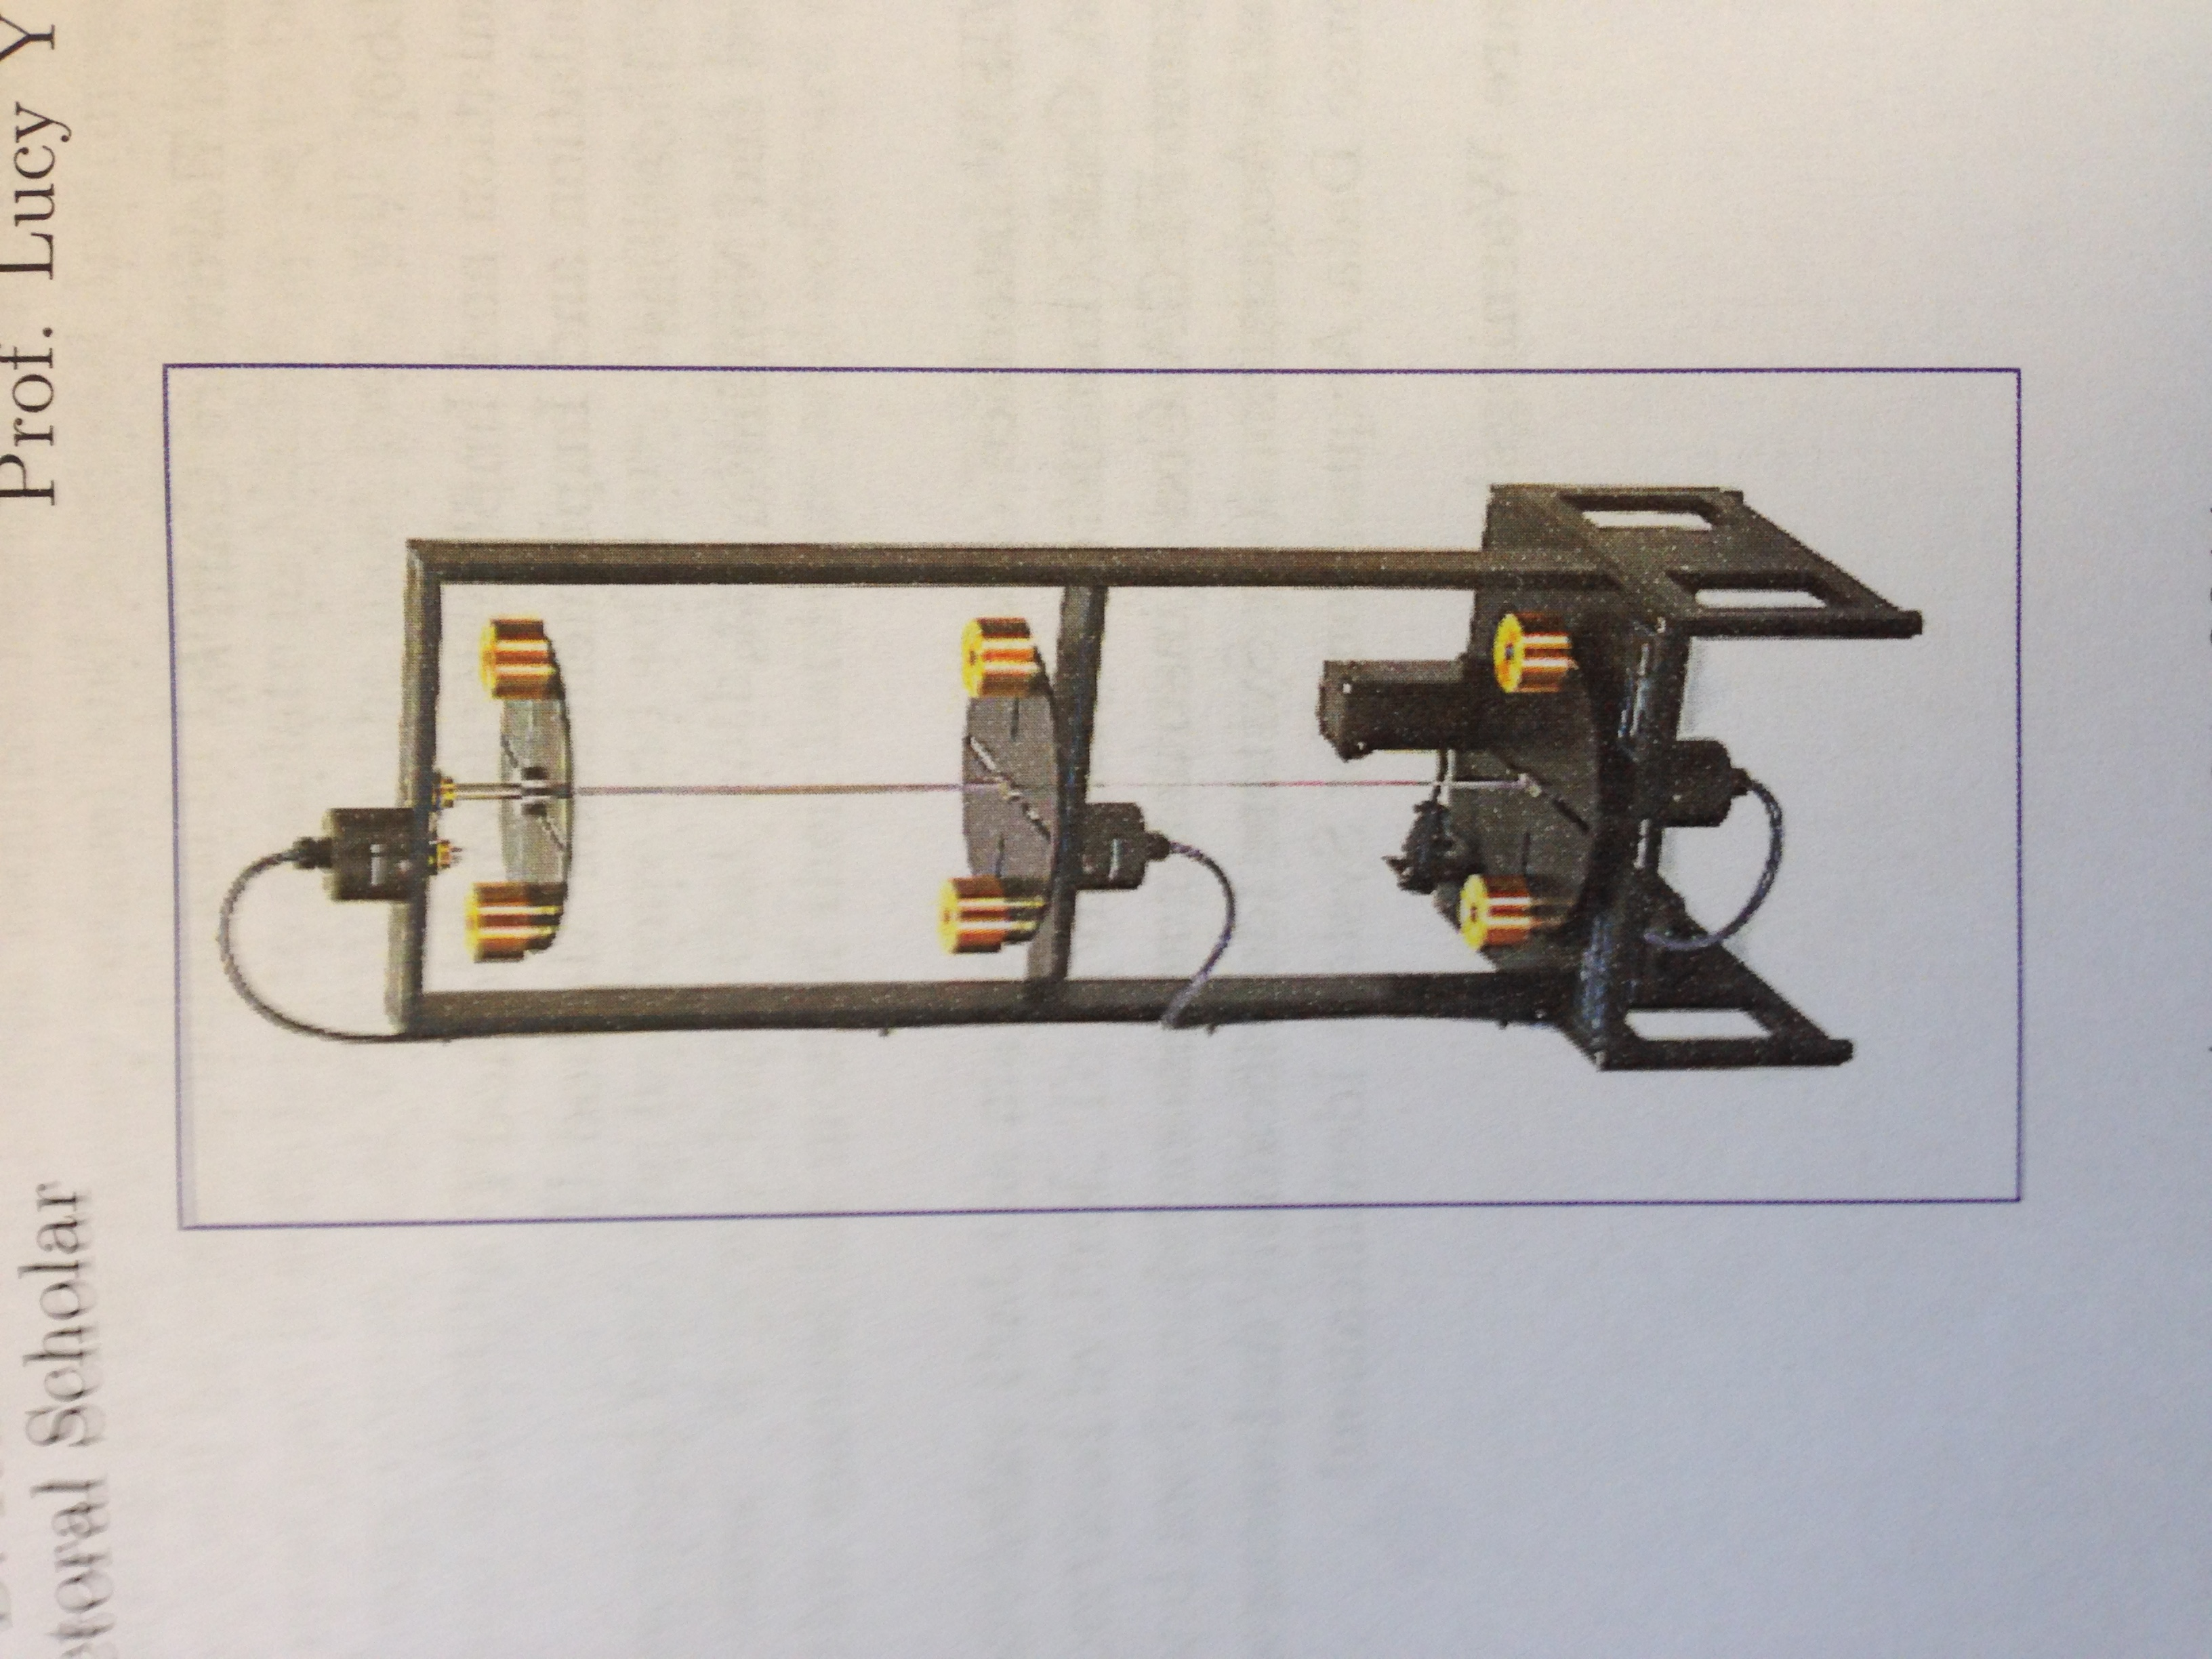
\includegraphics[trim={6cm 0 0 0},clip,angle=-90,origin=c,scale=0.1]{torsionSystem}
			\caption{Torsion Disc System}
	\end{figure}

\section{Setup}
	There are three main components that will be necessary for this lab.
	\begin{enumerate}
		\item LabView
		\item Matlab
		\item Torsion Disc System
	\end{enumerate}
	LabView and Matlab do not require any setup as they are installed on all lab computers. \\\\
	The torsion disc system must be configured for proper use. For this experiment the top two discs and any attached weights should be removed. After the weights and discs are removed the system cables can be connected.
	\subsection*{Steps}
	\begin{enumerate}
		\item loosen allen key screws on weights (do not remove weights on lower disc)
		\item remove weights
		\item loosen allen key screws on top two discs
		\item each disc detaches as two pieces
		\item remove the discs
		\item attach all labeled connectors
	\end{enumerate}

\section{LabView Intro}
	LabView is a high level program that will be used to control the torsion disc system. Data from the system will also be collected using LabView. The general idea is to build a block diagram of the system with appropriate input and output values as well as a configurable controller. In order to understand the operation of LabView it is useful to create a demo system before beginning work on the Torsion Disc system.
	\subsection{Simulation Loop}
		The below simulation loop was created in LabView. Transfer function blocks were used for the vehicle and controller while the reference and disturbance inputs use lookup tables. The output of the system is written to an external file.
		\begin{figure}[H]
			\centering
			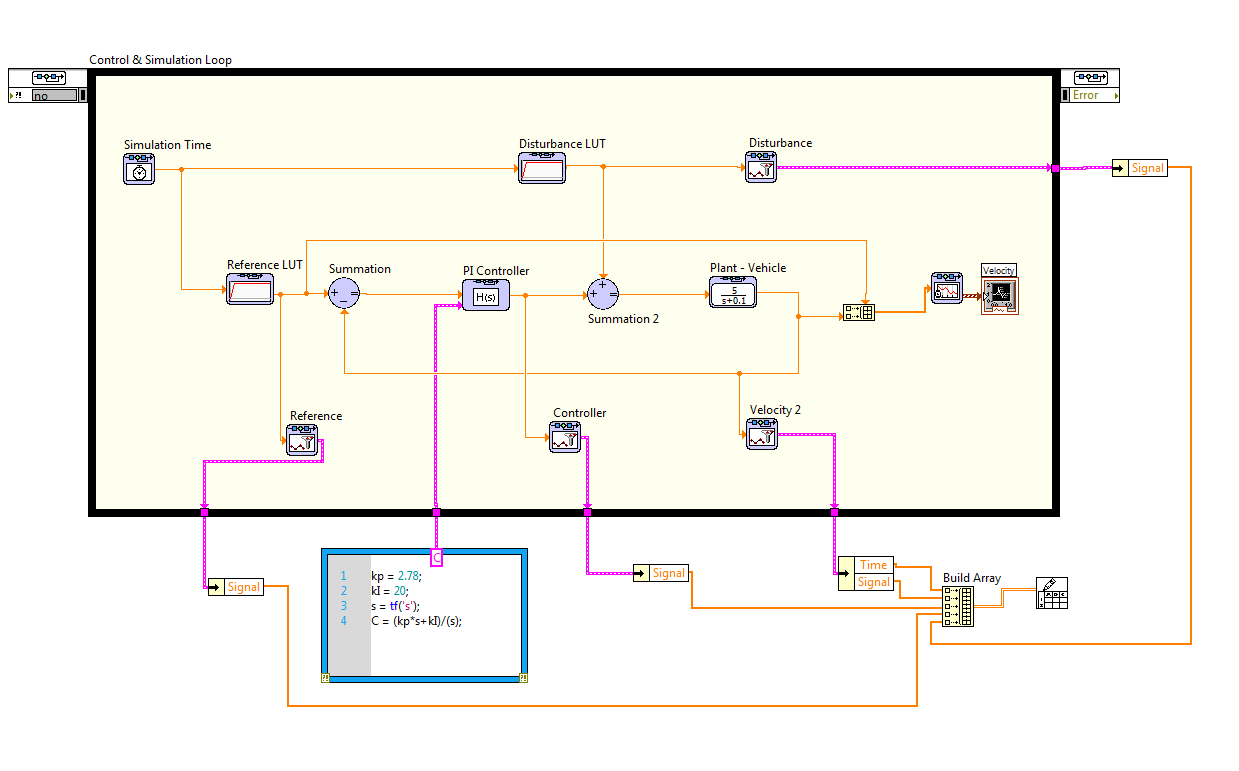
\includegraphics[scale=.5]{labviewIntro}
			\caption{LabView Model}
		\end{figure}
	\subsection{Controller Results}
		The collected results from the LabView simulations were taken and compared to the Simulink model used in LabX. As seen in the below plots, the results from LabView and simulink are comparable.
		\begin{figure}[H]
			\centering
			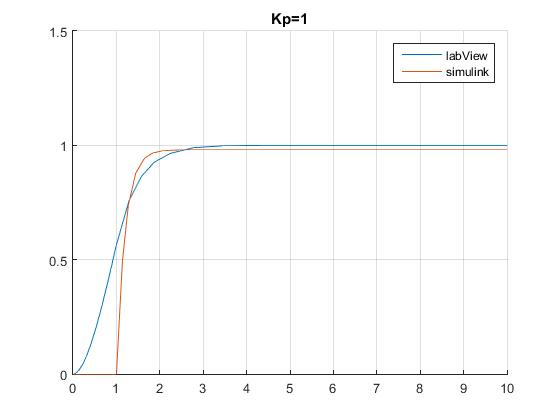
\includegraphics[scale=.5]{Kp1}
			\caption{LabView Model}
		\end{figure}	
	\subsection{Disturbance} 
		As a final experiment a disturbance was introduced to the LabView model that simulates a hill. The $P$ and $P_I$ values were chosen in order to produce a fast response with a small amount of overshoot and a reasonable settle time. In this case, values of $K_I=20$ and $K_I=60$ worked well.
		\begin{figure}[H]
			\centering
			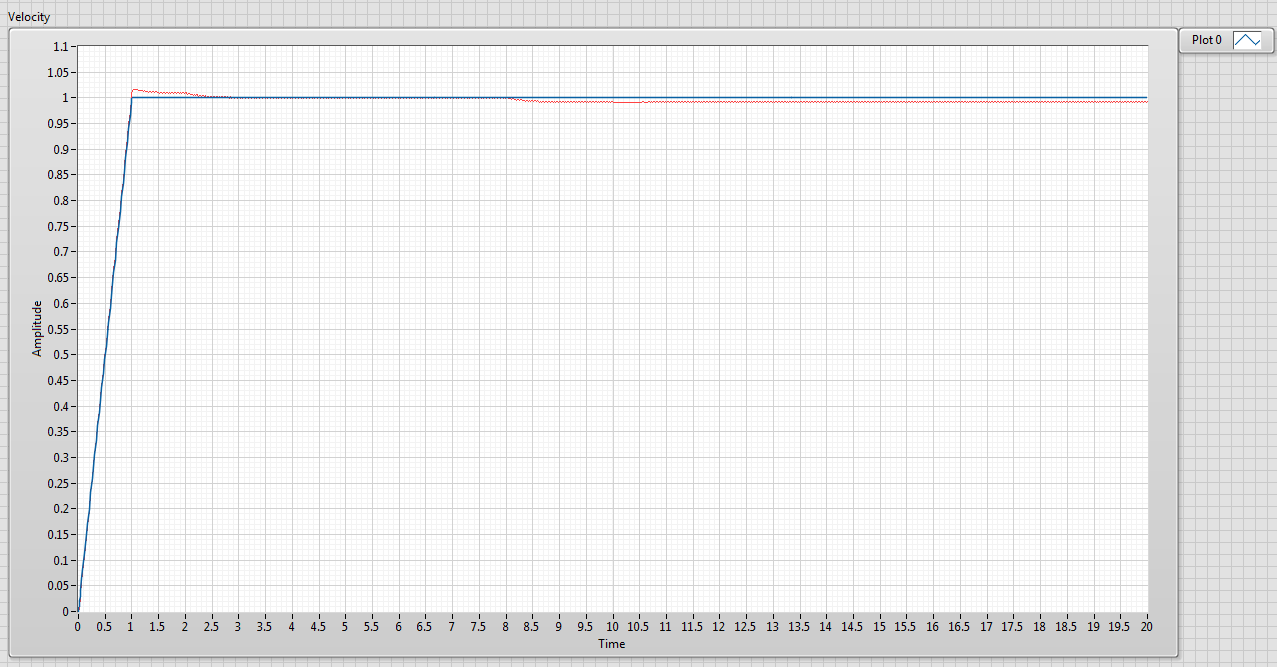
\includegraphics[scale=.4]{disturbance}
			\caption{Response with disturbance}
		\end{figure}

\section{Data Collection}
	To create a LTI model for the Torsion Disc system it is necessary to collect data that can be used to estimate system parameters. A LabView model is used to control the system and collect necessary data. The LabView model (shown below) was provided for this experiment and can be found on the ITLL share drive. Two experiments were conducted to collect the needed data.
	\begin{figure}[H]
			\centering
			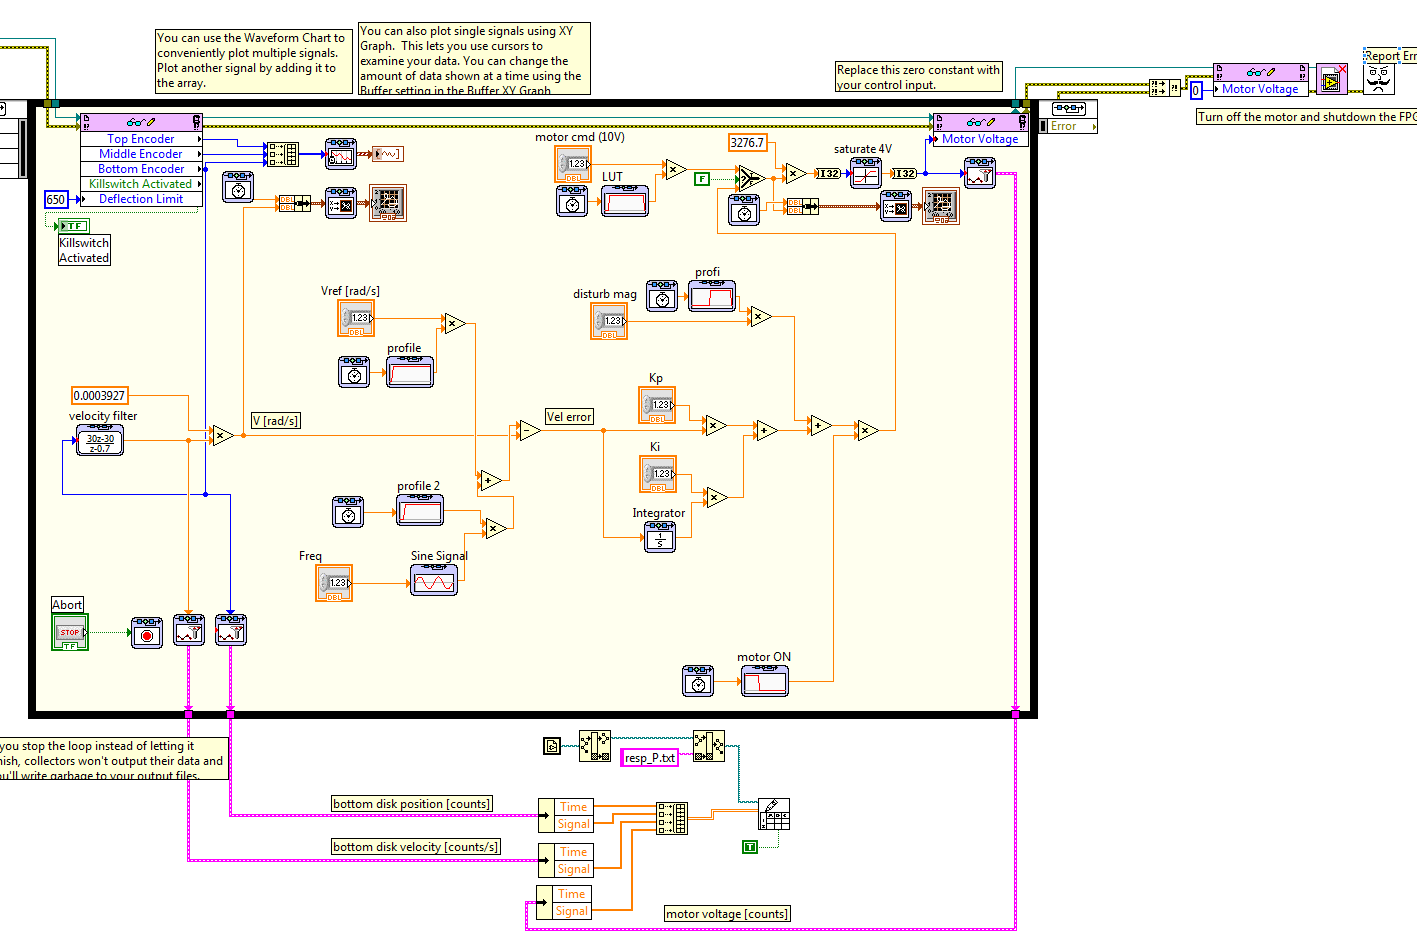
\includegraphics[scale=0.4]{labviewModel}
			\caption{Torsion Disc System}
	\end{figure}
	\subsection{No motor voltage}
		The first experiment is conducted with no power connected to the Torsion Disc motor. This is done in order to eliminate some of the parameters from the LTI model in order to estimate the value of $c$. Data is collected for three different weight positions which in turn give different inertia values for the system. The data is collected by first selecting a weight position and then manually spinning the disc by hand. \textbf{If only 2 weights are used they must be located along the hub split line.}
	\subsection*{Steps}
		\begin{enumerate}
			\item set the weights to a desired radius on the lower disc
			\item make sure the bolts holding the weights are firmly tightened
			\item begin data collection in LabView
			\item manually spin the disc and allow it to come to a stop
			\item data is saved as a text file
			\item change filename to reflect the weight position
		\end{enumerate}
			\textcolor{red}{add table showing weight positions}
	\subsection{Powered Torsion Disc System}
	The second data collection experiment is conducted with the power connected to the Torsion Disc system. In this case the values of various system parameters are adjusted in LabView while the weights remain in the same position. The collected data will then be used to create a proportional controller.
	\subsection*{Steps}
		\begin{enumerate}
			\item set reference speed to 3.14 rad/sec
			\item set disturbance to 0
			\item set $K_p$ to 1
			\item adjust experiment length to 12 seconds in order to collect data as the system comes to a stop
			\item \textbf{Ensure there is someone with their finger on the power of button in case the system goes unstable}
			\item turn the power on
			\item press the run button in LabView, data is saved as a text file
			\item rename file to reflect parameter values
			\item repeat for the values listed in below table
		\end{enumerate}
		\textcolor{red}{add table showing values we collected data for}

\section{LTI Model}
	The Torsion Disc system can be modeled as an LTI system with the below equation.
	\begin{equation} \label{eq:lti}
		J\dot{\omega}+c\omega=k_hu
	\end{equation}
	Where $J=\mbox{ total system inertia}$, $\omega=\mbox{ velocity rad/sec}$, $c=\mbox{ system drag}$, $k_h=\mbox{ hardware gain}$, $u=\mbox{ reference}$.

	\subsection{Estimating model values}
	Using equation \ref{eq:lti} and the collected data the value of $c$ can be estimated.

\section{Proportional Controller Design}

\end{document}